\documentclass[a4paper,10pt]{article}
\usepackage[utf8x]{inputenc}
\usepackage{amssymb,amsmath,amsthm}
\usepackage{hyperref}
\usepackage{cleveref}

% For Python syntax highlighting.
\usepackage{minted}

\usepackage[margin=1.0in]{geometry}


% For testing wether an argument of a macro is empty.
\usepackage{xifthen}
\usepackage{bm}

% Figures and subfigures.
\usepackage{subfig}
\usepackage{graphicx}

\newcommand{\dl}{\mathrm{d}\lambda}
\setlength{\parindent}{0cm}

%opening
\title{Development Journal and Specs of the MESLAS package
}

% % Macro file. We start with macros that are notation dependent, and hence
% susceptible to change.
% Purely static convenience mathematical macros (those that wont change) are
% grouped at the end of the file.

% Number of input dimensions nd and output dimensions no.
\newcommand{\no}{p}
\newcommand{\nd}{d}

% Mean and cov at time zero.
\newcommand{\mean}[1]{\mu
\left(#1\right)}
\newcommand{\covmat}[1]{K
\left(#1\right)}

% Product measure.
\newcommand{\productMeasure}{
d\nu^{\otimes}\left(\bm{u}\right)}

% Field value at x. Can either switch between parenthesis or subscripting.
% If no argument provided, then will just print xi.
\newcommand{\gp}[1][]{
    \ifthenelse{\isempty{#1}}
    {Z}
    {Z_{#1}}
}

% Covariance function k(., .).
\newcommand{\covFunc}[4]{k_{#2#4}\left(#1,#3\right)}

% Covariance matrix K = k(X, X).
\newcommand{\covMat}[4]{\bm{K}_{#2#4}(#1#3)}

% Mean function \mu(x).
\newcommand{\meanFunc}[2]{\mu_{#2}\left(#1\right)}

% Mean vector \mu(X).
\newcommand{\meanVec}[2]{\bm{\mu}_{#2}(#1)}

% Excursion probability in the set T^r.
\newcommand{\jointExcuProb}{
    \mathbb{P}\left(
    \gp[\bm{u}]\in T^r \right)
}

% In Proposition 1, the mean vector at the uu concatenation and the
% corresponding covariance matrix.
\newcommand{\meanUU}{
    \mu(\bm{u})
}

\newcommand{\covUU}{
    K\left(\bm{u},\bm{u}\right)
}

% ----------
% SEQUENTIAL
% ----------
% Probability distribution now (after 1 conditioning).
\newcommand{\currentProba}[1]{\mathbb{P}_{n}
\left(#1\right)}
% Probability distribution in the future (after 2 conditioning).
\newcommand{\futureProba}[1]{\mathbb{P}_{n+1}
\left(#1\right)}

% Same for expectations.
\newcommand{\currentExp}[1]{\mathbb{E}_{n}
\left[#1\right]}
\newcommand{\futureExp}[1]{\mathbb{E}_{n+1}
\left[#1\right]}

% For mean vectors.
\newcommand{\currentMean}[1]{\mu_{n}
\left(#1\right)}
\newcommand{\futureMean}[1]{\mu_{n+1}
\left(#1\right)}

% And covariance matrices.
\newcommand{\currentCov}[1]{K_{n}
\left(#1\right)}
\newcommand{\futureCov}[1]{K_{n+1}
\left(#1\right)}


% For nice expectations.
\usepackage{mathtools}
\newcommand{\expect}{\mathbb{E}\expectarg}
\DeclarePairedDelimiterX{\expectarg}[1]{[}{]}{%
  \ifnum\currentgrouptype=16 \else\begingroup\fi
  \activatebar#1
  \ifnum\currentgrouptype=16 \else\endgroup\fi
}

\newcommand{\innermid}{\nonscript\;\delimsize\vert\nonscript\;}
\newcommand{\activatebar}{%
  \begingroup\lccode`\~=`\|
  \lowercase{\endgroup\let~}\innermid
  \mathcode`|=\string"8000
}

% ----------
% General Mathematics (nothing to do with general notation choices.
% ----------
\DeclareMathOperator*{\argmin}{\arg\!\min}

% ----------
% OLD SEQUENTIAL
% ----------
% Probability distribution now (after 1 conditioning).
% \newcommand{\currentProba}[1]{\mathbb{P}_{\bm{Y}}
% \left(#1\right)}
% % Probability distribution in the future (after 2 conditioning).
% \newcommand{\futureProba}[1]{\mathbb{P}_{\bm{Y}\bm{Y}^{new}}
% \left(#1\right)}
% 
% % Same for expectations.
% \newcommand{\currentExp}[1]{\mathbb{E}_{\bm{Y}}
% \left[#1\right]}
% \newcommand{\futureExp}[1]{\mathbb{E}_{\bm{Y}\bm{Y}^{new}}
% \left[#1\right]}
% 
% % For mean vectors.
% \newcommand{\currentMean}[1]{\mu_{\bm{Y}}
% \left(#1\right)}
% \newcommand{\futureMean}[1]{\mu_{\bm{Y}\bm{Y}^{new}}
% \left(#1\right)}
% 
% % And covariance matrices.
% \newcommand{\currentCov}[1]{K_{\bm{Y}}
% \left(#1\right)}
% \newcommand{\futureCov}[1]{K_{\bm{Y}\bm{Y}^{new}}
% \left(#1\right)}

% Macro file. We start with macros that are notation dependent, and hence
% susceptible to change.
% Purely static convenience mathematical macros (those that wont change) are
% grouped at the end of the file.

% Number of input dimensions nd and output dimensions no.
\newcommand{\no}{p}
\newcommand{\nd}{d}

% Mean and cov at time zero.
\newcommand{\mean}[1]{\mu
\left(#1\right)}
\newcommand{\covmat}[1]{K
\left(#1\right)}

% Product measure.
\newcommand{\productMeasure}{
d\nu^{\otimes}\left(\bm{u}\right)}

% Field value at x. Can either switch between parenthesis or subscripting.
% If no argument provided, then will just print xi.
\newcommand{\gp}[1][]{
    \ifthenelse{\isempty{#1}}
    {Z}
    {Z_{#1}}
}

% Covariance function k(., .).
\newcommand{\covFunc}[4]{k_{#2#4}\left(#1,#3\right)}

% Covariance matrix K = k(X, X).
\newcommand{\covMat}[4]{\bm{K}_{#2#4}(#1#3)}

% Mean function \mu(x).
\newcommand{\meanFunc}[2]{\mu_{#2}\left(#1\right)}

% Mean vector \mu(X).
\newcommand{\meanVec}[2]{\bm{\mu}_{#2}(#1)}

% Excursion probability in the set T^r.
\newcommand{\jointExcuProb}{
    \mathbb{P}\left(
    \gp[\bm{u}]\in T^r \right)
}

% In Proposition 1, the mean vector at the uu concatenation and the
% corresponding covariance matrix.
\newcommand{\meanUU}{
    \mu(\bm{u})
}

\newcommand{\covUU}{
    K\left(\bm{u},\bm{u}\right)
}

% ----------
% SEQUENTIAL
% ----------
% Probability distribution now (after 1 conditioning).
\newcommand{\currentProba}[1]{\mathbb{P}_{n}
\left(#1\right)}
% Probability distribution in the future (after 2 conditioning).
\newcommand{\futureProba}[1]{\mathbb{P}_{n+1}
\left(#1\right)}

% Same for expectations.
\newcommand{\currentExp}[1]{\mathbb{E}_{n}
\left[#1\right]}
\newcommand{\futureExp}[1]{\mathbb{E}_{n+1}
\left[#1\right]}

% For mean vectors.
\newcommand{\currentMean}[1]{\mu_{n}
\left(#1\right)}
\newcommand{\futureMean}[1]{\mu_{n+1}
\left(#1\right)}

% And covariance matrices.
\newcommand{\currentCov}[1]{K_{n}
\left(#1\right)}
\newcommand{\futureCov}[1]{K_{n+1}
\left(#1\right)}


% For nice expectations.
\usepackage{mathtools}
\newcommand{\expect}{\mathbb{E}\expectarg}
\DeclarePairedDelimiterX{\expectarg}[1]{[}{]}{%
  \ifnum\currentgrouptype=16 \else\begingroup\fi
  \activatebar#1
  \ifnum\currentgrouptype=16 \else\endgroup\fi
}

\newcommand{\innermid}{\nonscript\;\delimsize\vert\nonscript\;}
\newcommand{\activatebar}{%
  \begingroup\lccode`\~=`\|
  \lowercase{\endgroup\let~}\innermid
  \mathcode`|=\string"8000
}

% ----------
% General Mathematics (nothing to do with general notation choices.
% ----------
\DeclareMathOperator*{\argmin}{\arg\!\min}

% ----------
% OLD SEQUENTIAL
% ----------
% Probability distribution now (after 1 conditioning).
% \newcommand{\currentProba}[1]{\mathbb{P}_{\bm{Y}}
% \left(#1\right)}
% % Probability distribution in the future (after 2 conditioning).
% \newcommand{\futureProba}[1]{\mathbb{P}_{\bm{Y}\bm{Y}^{new}}
% \left(#1\right)}
% 
% % Same for expectations.
% \newcommand{\currentExp}[1]{\mathbb{E}_{\bm{Y}}
% \left[#1\right]}
% \newcommand{\futureExp}[1]{\mathbb{E}_{\bm{Y}\bm{Y}^{new}}
% \left[#1\right]}
% 
% % For mean vectors.
% \newcommand{\currentMean}[1]{\mu_{\bm{Y}}
% \left(#1\right)}
% \newcommand{\futureMean}[1]{\mu_{\bm{Y}\bm{Y}^{new}}
% \left(#1\right)}
% 
% % And covariance matrices.
% \newcommand{\currentCov}[1]{K_{\bm{Y}}
% \left(#1\right)}
% \newcommand{\futureCov}[1]{K_{\bm{Y}\bm{Y}^{new}}
% \left(#1\right)}


\begin{document}
\maketitle

\section{General Considerations}
The MESLAS package (\textbf{M}ulti-variate \textbf{E}xcursion \textbf{S}et \textbf{L}earning by \textbf{A}daptive \textbf{S}ampling) is a toolbox for simulation and prediction of mulitivariate Gaussian random fields.\\

The setup of the package is the following: $\gp$ is a $\no$-dimensional random
field on a domain $\nd$-dimensional
domain $D$.

Our philosophy is to always specify spatial location and response indices
together. That is, one should always specify \textbf{where} and \textbf{what}.

Spatial locations are denoted by $s$ and response indices by $\ell$. We will
use boldface (or, in the code, alternatively uppercase or plurals) to denote
vectors of such objects.

\medskip
A generalized sampling location is thus entirely defined by specifying two vectors
\begin{align*}
    \bm{s} &= \left(s_1, ..., s_n\right)\in D^n\\
    \bm{\ell} &= \left(\ell_1, ..., \ell_n\right) \in \lbrace 1, ..., \no
    \rbrace^n
\end{align*}
We will refer to $n$ as the \textit{dimension} of the generalized sampling
location and usually just talk of location, using the word \textit{spatial
location} when we want to specifically refer to points in $D$. Also, we will
use boldface $x$ as a shortcut to refer to the couple $\left(\bm{s},
\bm{\ell}\right)$ of spatial location vector and response index vector.
The shortcut notation $\gp[\bm{x}]$ thus refers to the
vector
\[
    \gp[\bm{x}]:=\left(\gp[s_1]^{\ell_1}, ..., \gp[s_n]^{\ell_n}\right) \in
    \mathbb{R}^n.
\]

\subsection{Covariance Model}
We assume a factor model which is the product of a stationary spatial component
with a response-index component
\begin{equation}
    \textrm{Cov}\left(\gp[s]^i, \gp[t]^j\right) = k\left(s - t\right)
    \gamma\left(i, j\right).
\end{equation}

This makes implementation easier, since then, to compute the covariance matrix
of a generalized observations $\left(S, L\right)$, we first compute the
pairwise distance matrix
\[
    H = \textrm{cdist}\left(S,S, p=2\right) = \begin{pmatrix}
        ||s_1 - s_1|| & \dots & ||s_1 - s_n||\\
        \vdots &  & \vdots \\
        ||s_n - s_1|| & \dots & ||s_n - s_n||\\
    \end{pmatrix}
\]
which can then be feeded to a vectorized stationary covariance function to get
$K(H)$.

For the response index part, we compute $L_1, L_2=\textrm{meshgrid}\left(L,
L\right)$ which yields
\begin{align*}
    L_1 =  \begin{pmatrix}
        l_1 & \dots & l_1\\
        \vdots &  & \vdots \\
        l_n & \dots & l_n\\
    \end{pmatrix}
    &,~ 
    L_2 =  \begin{pmatrix}
        l_1 & \dots & l_n\\
        \vdots &  & \vdots \\
        l_1 & \dots & l_n\\
    \end{pmatrix}
\end{align*}
and then feed it to a vectorized cross-covariance function $\gamma(L_1, L_2)$.
Finally, we get the covariance matrix by elementwise multiplication
\[
    K = K\left(H\right) \odot \gamma\left(L_1, L_2\right)
\]

\subsection{Cross-Covariance Models}
We here review different usual models for the cross-covariance part $\gamma(.,
.)$ of the covariance function. Recall that this is the part that specifies how
different components of the response vector at one fixed location interact.

\medskip
The simplest model we will consider is \textbf{uniform mixing}. In this model,
all components interact with the same coupling $\gamma_0$:
\begin{equation}
    \gamma(l, m) = \begin{cases} \sigma_l^2,~ l=m\\ 
        \gamma_0\sigma_l\sigma_m,~l\neq m
    \end{cases}
\end{equation}
and $\sigma_1^2, ..., \sigma_{\no}^2$ are the variances of the individual
components.

\subsection{Implementation Details}
ATTENTION: torch.meshgrid behaves differently than numpy's one.
First of all, it takes single dimensional vectors.
\[
    L=(1,2,3,4),~ \textrm{torch.meshgrid}(L,L)=
    \begin{pmatrix}
        1 & \dots & 1\\
        \vdots &  & \vdots \\
        n & \dots & n\\
    \end{pmatrix}
    ,~ 
    \begin{pmatrix}
        1 & \dots & n\\
        \vdots &  & \vdots \\
        1 & \dots & n\\
    \end{pmatrix}
\]

\subsection{Mean Module}
\subsection{Covariance Module}
\subsection{Gaussian Random Field Class and Sampling}
\subsection{Gridding}

\newpage

\section{Example Run}
We consider a $2$-dimensional GRF on a a $2$-dimensional $100\times 100$ regular grid on
$[0,1]^2$. The GRF has a factor covariance model, where the spatial part is a
Mat\'{e}rn $3/2$ with unit variance and lengthscale $\lambda_0 = 0.1$. The
cross-covariance is a uniform mixing with parameters
\[
    \sigma_1^2 = 0.25,~\sigma_2^2 = 0.6, \gamma_0 = 0.3
\]
and the mean function is a constant one with $\mu_0=(1, -2)$.
\medskip

The plot below shows one realization of the field on the full grid.
\begin{figure}[tbh!p]
\centering
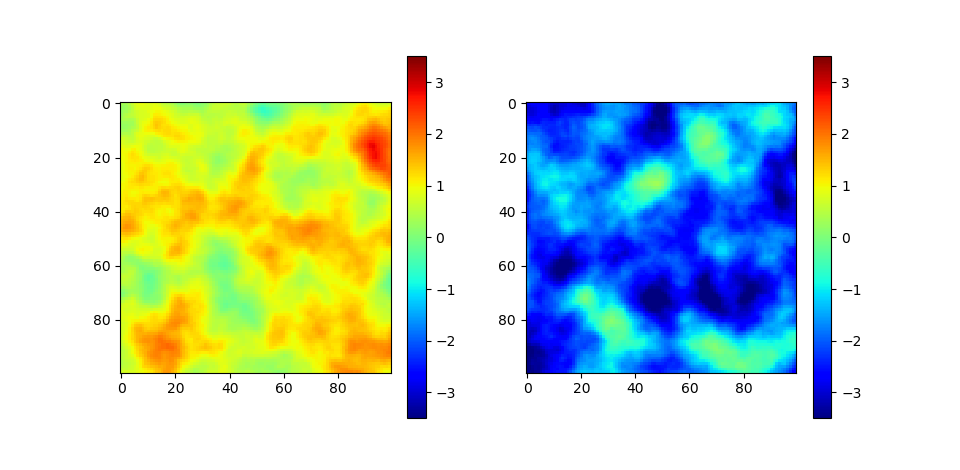
\includegraphics[scale=0.65]{images/sample_low_correlation.png}
\caption{Simulated first (left) and second (right) component of the field.}
\end{figure}

We can also increase the cross-correlation factor $\gamma_0$ to $0.9$ to see
its effect.
\begin{figure}[tbh!p]
\centering
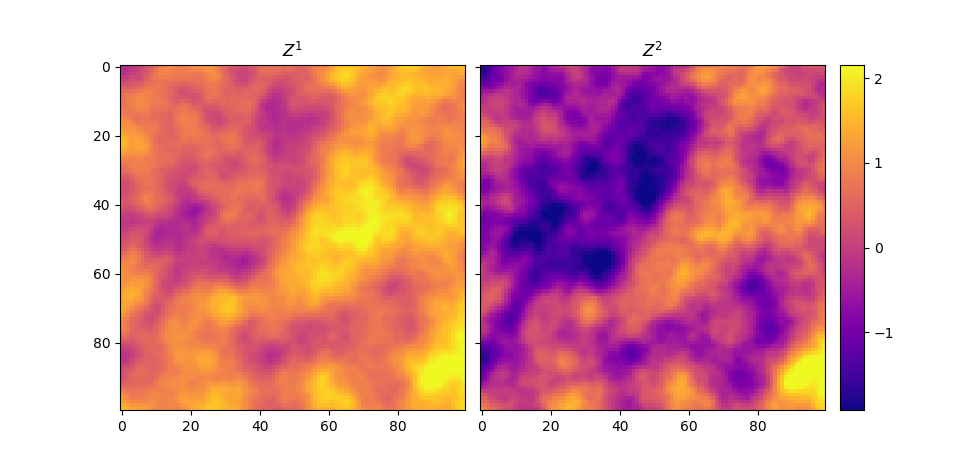
\includegraphics[scale=0.65]{images/sample_high_correlation.png}
\caption{Simulation of highly cross-correlated field.}
\end{figure}

\newpage
The code below shows how simple it is to sample a multivariate GRF using MESLAS.
\usemintedstyle{tango}
\inputminted{python}{example_sample.py}

\section{Co-Kriging}
Cokriging is also implemented in full generality (heterotopic) in MESLAS. The package also provides conditional simulations. Plots below show an example of cokriging and conditional simulation. The GRF is the same as in the previous section, with a high cross-correlation $\gamma_0=0.9$.

\begin{figure}[tbh!p]
\centering
\subfloat[Conditional mean]{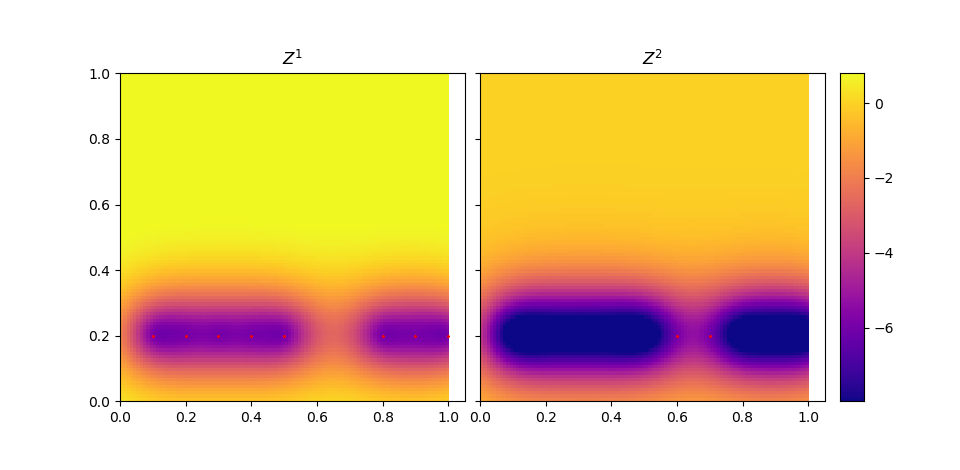
\includegraphics[scale=0.6]{images/cond_mean_high_corr.png}}\\
\subfloat[Conditional realisation]{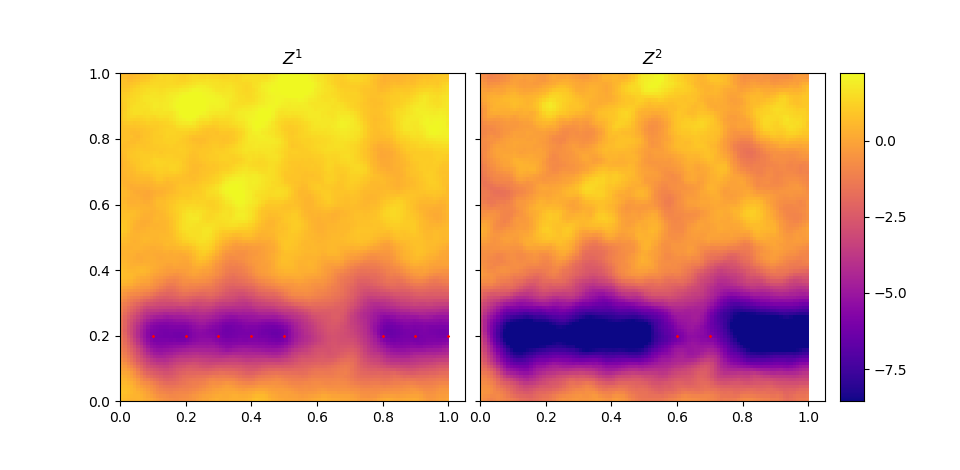
\includegraphics[scale=0.6]{images/cond_realisation_high_corr.png}}
\caption{Example of co-kriging a 2-dimensional GRF with MESLAS, observation locations in red.}
\label{fig:example_inv_prob}
\end{figure}

\newpage

\section{Coverage Function}
We compute the $p$-dimensional CDF using the MVNORM package of Sebastion Marmin. We re-packaged it for streamlined distribution via PiPy. The implementation is $3$ times faster than barebone PyTorch (in dimension 2). It is also vectorized over the batch dimension.

Below we demonstrate the computation of the coverage function for excursion
above $t=\left(-1.0, -1.0\right)$.
\begin{figure}[tbh!p]
\centering
\subfloat[Conditional mean]{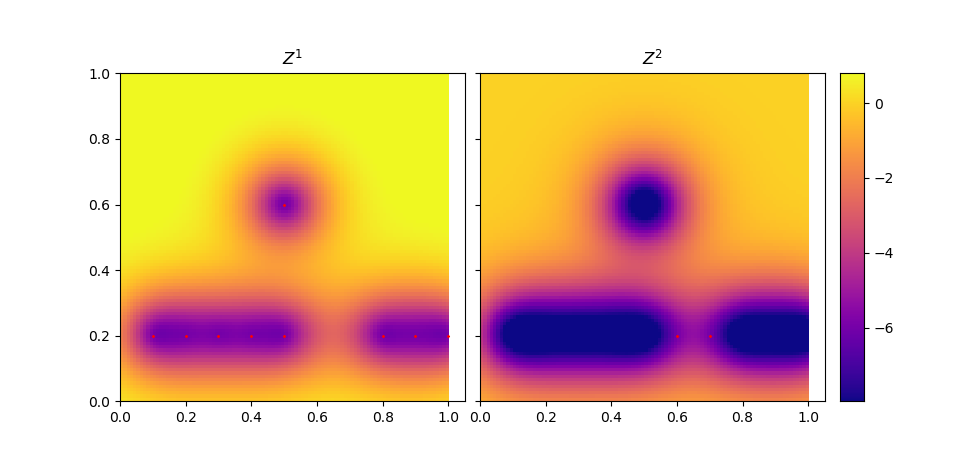
\includegraphics[scale=0.6]{images/coverage_mean.png}}\\
\subfloat[Sample conditional realisation]{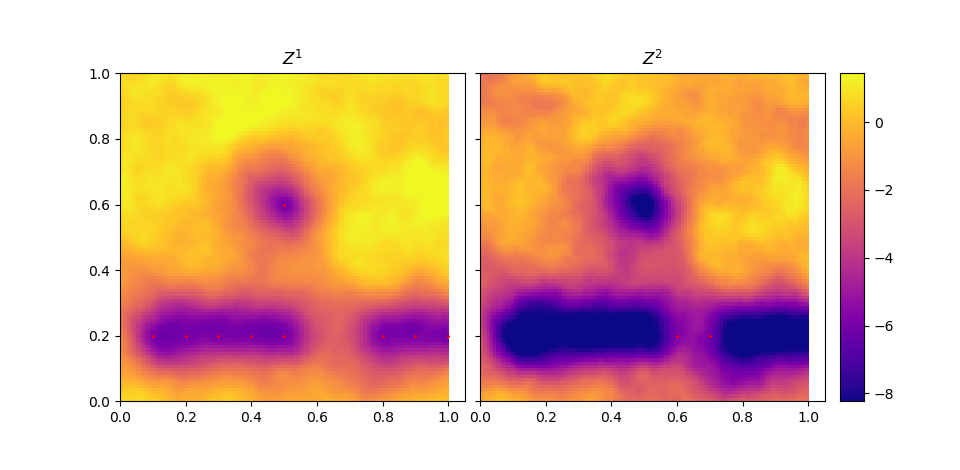
\includegraphics[scale=0.6]{images/coverage_realisation.png}}\\
\subfloat[Conditional Coverage Function]{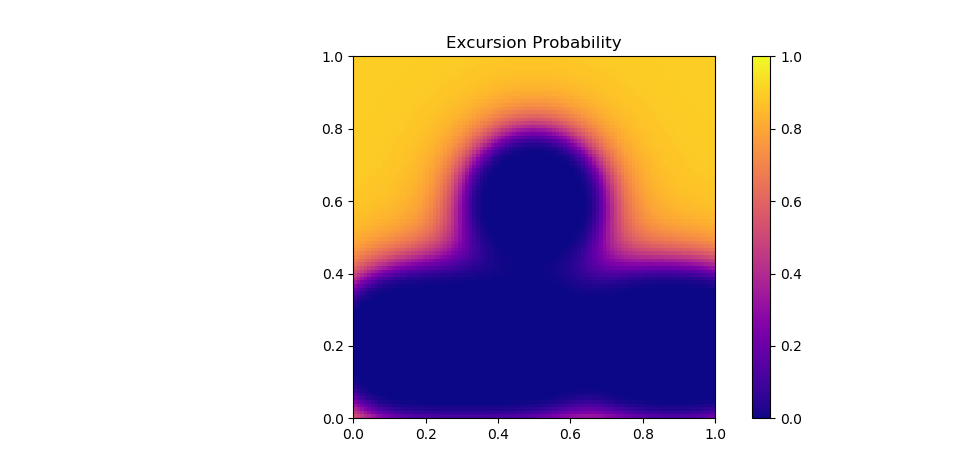
\includegraphics[scale=0.6]{images/coverage_coverage.png}}
\caption{Diagnostics of problems in computation of the coverage function.}
\label{fig:example_inv_prob}
\end{figure}

\subsection{Illustrations}
The agreed-upon goal was to produce plots to illustrate multivariate excursion
sets vs univariate.

I suggest we do that by trying to replace figure 4 in the paper.
So: sample unconditionally, illustrate various excursions, krig using this
realisation, plot coverages.

\begin{figure}[tbh!p]
\centering
\subfloat[Simulated Realisation]{\includegraphics[scale=0.6]{images/Figure4/cond_realisation.png}}\\
\subfloat[Cokriging Mean (observation locations in red)]{\includegraphics[scale=0.6]{images/Figure4/cond_mean.png}}\\
\subfloat[Coverage Function]{
	\includegraphics[scale=0.45]{images/Figure4/salinity_excu.png}
	\includegraphics[scale=0.45]{images/Figure4/temperature_excu.png}
	\includegraphics[scale=0.45]{images/Figure4/joint_excu.png}}
\caption{Diagnostics of problems in computation of the coverage function.}
\label{fig:example_inv_prob}
\end{figure}

\section{Hardware/Software Specifications}
The AUV feature a Nvidia TX1 with ubuntu 16.04. Current programs use Python
2.7, but 3.7 can be used.
In order to run 3.7, we have to run
another backseat-driver (responsible for sending waypoints to the low-leve
controllers).


\end{document}
